\documentclass[11pt]{article}

    \usepackage[breakable]{tcolorbox}
    \usepackage{parskip} % Stop auto-indenting (to mimic markdown behaviour)
    
    \newcommand{\ind}{\raisebox{0.05em}{\rotatebox[origin=c]{90}{$\models$}}}

    % Basic figure setup, for now with no caption control since it's done
    % automatically by Pandoc (which extracts ![](path) syntax from Markdown).
    \usepackage{graphicx}
    % Maintain compatibility with old templates. Remove in nbconvert 6.0
    \let\Oldincludegraphics\includegraphics
    % Ensure that by default, figures have no caption (until we provide a
    % proper Figure object with a Caption API and a way to capture that
    % in the conversion process - todo).
    \usepackage{caption}
    \DeclareCaptionFormat{nocaption}{}
    \captionsetup{format=nocaption,aboveskip=0pt,belowskip=0pt}

    \usepackage{float}
    \floatplacement{figure}{H} % forces figures to be placed at the correct location
    \usepackage{xcolor} % Allow colors to be defined
    \usepackage{enumerate} % Needed for markdown enumerations to work
    \usepackage{geometry} % Used to adjust the document margins
    \usepackage{amsmath} % Equations
    \usepackage{amssymb} % Equations
    \usepackage{textcomp} % defines textquotesingle
    % Hack from http://tex.stackexchange.com/a/47451/13684:
    \AtBeginDocument{%
        \def\PYZsq{\textquotesingle}% Upright quotes in Pygmentized code
    }
    \usepackage{upquote} % Upright quotes for verbatim code
    \usepackage{eurosym} % defines \euro

    \usepackage{iftex}
    \ifPDFTeX
        \usepackage[T1]{fontenc}
        \IfFileExists{alphabeta.sty}{
              \usepackage{alphabeta}
          }{
              \usepackage[mathletters]{ucs}
              \usepackage[utf8x]{inputenc}
          }
    \else
        \usepackage{fontspec}
        \usepackage{unicode-math}
    \fi

    \usepackage{fancyvrb} % verbatim replacement that allows latex
    \usepackage{grffile} % extends the file name processing of package graphics
                         % to support a larger range
    \makeatletter % fix for old versions of grffile with XeLaTeX
    \@ifpackagelater{grffile}{2019/11/01}
    {
      % Do nothing on new versions
    }
    {
      \def\Gread@@xetex#1{%
        \IfFileExists{"\Gin@base".bb}%
        {\Gread@eps{\Gin@base.bb}}%
        {\Gread@@xetex@aux#1}%
      }
    }
    \makeatother
    \usepackage[Export]{adjustbox} % Used to constrain images to a maximum size
    \adjustboxset{max size={0.9\linewidth}{0.9\paperheight}}

    % The hyperref package gives us a pdf with properly built
    % internal navigation ('pdf bookmarks' for the table of contents,
    % internal cross-reference links, web links for URLs, etc.)
    \usepackage{hyperref}
    % The default LaTeX title has an obnoxious amount of whitespace. By default,
    % titling removes some of it. It also provides customization options.
    \usepackage{titling}
    \usepackage{longtable} % longtable support required by pandoc >1.10
    \usepackage{booktabs}  % table support for pandoc > 1.12.2
    \usepackage{array}     % table support for pandoc >= 2.11.3
    \usepackage{calc}      % table minipage width calculation for pandoc >= 2.11.1
    \usepackage[inline]{enumitem} % IRkernel/repr support (it uses the enumerate* environment)
    \usepackage[normalem]{ulem} % ulem is needed to support strikethroughs (\sout)
                                % normalem makes italics be italics, not underlines
    \usepackage{mathrsfs}
    

    
    % Colors for the hyperref package
    \definecolor{urlcolor}{rgb}{0,.145,.698}
    \definecolor{linkcolor}{rgb}{.71,0.21,0.01}
    \definecolor{citecolor}{rgb}{.12,.54,.11}

    % ANSI colors
    \definecolor{ansi-black}{HTML}{3E424D}
    \definecolor{ansi-black-intense}{HTML}{282C36}
    \definecolor{ansi-red}{HTML}{E75C58}
    \definecolor{ansi-red-intense}{HTML}{B22B31}
    \definecolor{ansi-green}{HTML}{00A250}
    \definecolor{ansi-green-intense}{HTML}{007427}
    \definecolor{ansi-yellow}{HTML}{DDB62B}
    \definecolor{ansi-yellow-intense}{HTML}{B27D12}
    \definecolor{ansi-blue}{HTML}{208FFB}
    \definecolor{ansi-blue-intense}{HTML}{0065CA}
    \definecolor{ansi-magenta}{HTML}{D160C4}
    \definecolor{ansi-magenta-intense}{HTML}{A03196}
    \definecolor{ansi-cyan}{HTML}{60C6C8}
    \definecolor{ansi-cyan-intense}{HTML}{258F8F}
    \definecolor{ansi-white}{HTML}{C5C1B4}
    \definecolor{ansi-white-intense}{HTML}{A1A6B2}
    \definecolor{ansi-default-inverse-fg}{HTML}{FFFFFF}
    \definecolor{ansi-default-inverse-bg}{HTML}{000000}

    % common color for the border for error outputs.
    \definecolor{outerrorbackground}{HTML}{FFDFDF}

    % commands and environments needed by pandoc snippets
    % extracted from the output of `pandoc -s`
    \providecommand{\tightlist}{%
      \setlength{\itemsep}{0pt}\setlength{\parskip}{0pt}}
    \DefineVerbatimEnvironment{Highlighting}{Verbatim}{commandchars=\\\{\}}
    % Add ',fontsize=\small' for more characters per line
    \newenvironment{Shaded}{}{}
    \newcommand{\KeywordTok}[1]{\textcolor[rgb]{0.00,0.44,0.13}{\textbf{{#1}}}}
    \newcommand{\DataTypeTok}[1]{\textcolor[rgb]{0.56,0.13,0.00}{{#1}}}
    \newcommand{\DecValTok}[1]{\textcolor[rgb]{0.25,0.63,0.44}{{#1}}}
    \newcommand{\BaseNTok}[1]{\textcolor[rgb]{0.25,0.63,0.44}{{#1}}}
    \newcommand{\FloatTok}[1]{\textcolor[rgb]{0.25,0.63,0.44}{{#1}}}
    \newcommand{\CharTok}[1]{\textcolor[rgb]{0.25,0.44,0.63}{{#1}}}
    \newcommand{\StringTok}[1]{\textcolor[rgb]{0.25,0.44,0.63}{{#1}}}
    \newcommand{\CommentTok}[1]{\textcolor[rgb]{0.38,0.63,0.69}{\textit{{#1}}}}
    \newcommand{\OtherTok}[1]{\textcolor[rgb]{0.00,0.44,0.13}{{#1}}}
    \newcommand{\AlertTok}[1]{\textcolor[rgb]{1.00,0.00,0.00}{\textbf{{#1}}}}
    \newcommand{\FunctionTok}[1]{\textcolor[rgb]{0.02,0.16,0.49}{{#1}}}
    \newcommand{\RegionMarkerTok}[1]{{#1}}
    \newcommand{\ErrorTok}[1]{\textcolor[rgb]{1.00,0.00,0.00}{\textbf{{#1}}}}
    \newcommand{\NormalTok}[1]{{#1}}

    % Additional commands for more recent versions of Pandoc
    \newcommand{\ConstantTok}[1]{\textcolor[rgb]{0.53,0.00,0.00}{{#1}}}
    \newcommand{\SpecialCharTok}[1]{\textcolor[rgb]{0.25,0.44,0.63}{{#1}}}
    \newcommand{\VerbatimStringTok}[1]{\textcolor[rgb]{0.25,0.44,0.63}{{#1}}}
    \newcommand{\SpecialStringTok}[1]{\textcolor[rgb]{0.73,0.40,0.53}{{#1}}}
    \newcommand{\ImportTok}[1]{{#1}}
    \newcommand{\DocumentationTok}[1]{\textcolor[rgb]{0.73,0.13,0.13}{\textit{{#1}}}}
    \newcommand{\AnnotationTok}[1]{\textcolor[rgb]{0.38,0.63,0.69}{\textbf{\textit{{#1}}}}}
    \newcommand{\CommentVarTok}[1]{\textcolor[rgb]{0.38,0.63,0.69}{\textbf{\textit{{#1}}}}}
    \newcommand{\VariableTok}[1]{\textcolor[rgb]{0.10,0.09,0.49}{{#1}}}
    \newcommand{\ControlFlowTok}[1]{\textcolor[rgb]{0.00,0.44,0.13}{\textbf{{#1}}}}
    \newcommand{\OperatorTok}[1]{\textcolor[rgb]{0.40,0.40,0.40}{{#1}}}
    \newcommand{\BuiltInTok}[1]{{#1}}
    \newcommand{\ExtensionTok}[1]{{#1}}
    \newcommand{\PreprocessorTok}[1]{\textcolor[rgb]{0.74,0.48,0.00}{{#1}}}
    \newcommand{\AttributeTok}[1]{\textcolor[rgb]{0.49,0.56,0.16}{{#1}}}
    \newcommand{\InformationTok}[1]{\textcolor[rgb]{0.38,0.63,0.69}{\textbf{\textit{{#1}}}}}
    \newcommand{\WarningTok}[1]{\textcolor[rgb]{0.38,0.63,0.69}{\textbf{\textit{{#1}}}}}


    % Define a nice break command that doesn't care if a line doesn't already
    % exist.
    \def\br{\hspace*{\fill} \\* }
    % Math Jax compatibility definitions
    \def\gt{>}
    \def\lt{<}
    \let\Oldtex\TeX
    \let\Oldlatex\LaTeX
    \renewcommand{\TeX}{\textrm{\Oldtex}}
    \renewcommand{\LaTeX}{\textrm{\Oldlatex}}
    % Document parameters
    % Document title
    \title{CFRM 505 Homework 1}
    \author{Eunki Chung \\
    \small{eunkich@uw.edu}}
    
    
    
    
    
% Pygments definitions
\makeatletter
\def\PY@reset{\let\PY@it=\relax \let\PY@bf=\relax%
    \let\PY@ul=\relax \let\PY@tc=\relax%
    \let\PY@bc=\relax \let\PY@ff=\relax}
\def\PY@tok#1{\csname PY@tok@#1\endcsname}
\def\PY@toks#1+{\ifx\relax#1\empty\else%
    \PY@tok{#1}\expandafter\PY@toks\fi}
\def\PY@do#1{\PY@bc{\PY@tc{\PY@ul{%
    \PY@it{\PY@bf{\PY@ff{#1}}}}}}}
\def\PY#1#2{\PY@reset\PY@toks#1+\relax+\PY@do{#2}}

\@namedef{PY@tok@w}{\def\PY@tc##1{\textcolor[rgb]{0.73,0.73,0.73}{##1}}}
\@namedef{PY@tok@c}{\let\PY@it=\textit\def\PY@tc##1{\textcolor[rgb]{0.24,0.48,0.48}{##1}}}
\@namedef{PY@tok@cp}{\def\PY@tc##1{\textcolor[rgb]{0.61,0.40,0.00}{##1}}}
\@namedef{PY@tok@k}{\let\PY@bf=\textbf\def\PY@tc##1{\textcolor[rgb]{0.00,0.50,0.00}{##1}}}
\@namedef{PY@tok@kp}{\def\PY@tc##1{\textcolor[rgb]{0.00,0.50,0.00}{##1}}}
\@namedef{PY@tok@kt}{\def\PY@tc##1{\textcolor[rgb]{0.69,0.00,0.25}{##1}}}
\@namedef{PY@tok@o}{\def\PY@tc##1{\textcolor[rgb]{0.40,0.40,0.40}{##1}}}
\@namedef{PY@tok@ow}{\let\PY@bf=\textbf\def\PY@tc##1{\textcolor[rgb]{0.67,0.13,1.00}{##1}}}
\@namedef{PY@tok@nb}{\def\PY@tc##1{\textcolor[rgb]{0.00,0.50,0.00}{##1}}}
\@namedef{PY@tok@nf}{\def\PY@tc##1{\textcolor[rgb]{0.00,0.00,1.00}{##1}}}
\@namedef{PY@tok@nc}{\let\PY@bf=\textbf\def\PY@tc##1{\textcolor[rgb]{0.00,0.00,1.00}{##1}}}
\@namedef{PY@tok@nn}{\let\PY@bf=\textbf\def\PY@tc##1{\textcolor[rgb]{0.00,0.00,1.00}{##1}}}
\@namedef{PY@tok@ne}{\let\PY@bf=\textbf\def\PY@tc##1{\textcolor[rgb]{0.80,0.25,0.22}{##1}}}
\@namedef{PY@tok@nv}{\def\PY@tc##1{\textcolor[rgb]{0.10,0.09,0.49}{##1}}}
\@namedef{PY@tok@no}{\def\PY@tc##1{\textcolor[rgb]{0.53,0.00,0.00}{##1}}}
\@namedef{PY@tok@nl}{\def\PY@tc##1{\textcolor[rgb]{0.46,0.46,0.00}{##1}}}
\@namedef{PY@tok@ni}{\let\PY@bf=\textbf\def\PY@tc##1{\textcolor[rgb]{0.44,0.44,0.44}{##1}}}
\@namedef{PY@tok@na}{\def\PY@tc##1{\textcolor[rgb]{0.41,0.47,0.13}{##1}}}
\@namedef{PY@tok@nt}{\let\PY@bf=\textbf\def\PY@tc##1{\textcolor[rgb]{0.00,0.50,0.00}{##1}}}
\@namedef{PY@tok@nd}{\def\PY@tc##1{\textcolor[rgb]{0.67,0.13,1.00}{##1}}}
\@namedef{PY@tok@s}{\def\PY@tc##1{\textcolor[rgb]{0.73,0.13,0.13}{##1}}}
\@namedef{PY@tok@sd}{\let\PY@it=\textit\def\PY@tc##1{\textcolor[rgb]{0.73,0.13,0.13}{##1}}}
\@namedef{PY@tok@si}{\let\PY@bf=\textbf\def\PY@tc##1{\textcolor[rgb]{0.64,0.35,0.47}{##1}}}
\@namedef{PY@tok@se}{\let\PY@bf=\textbf\def\PY@tc##1{\textcolor[rgb]{0.67,0.36,0.12}{##1}}}
\@namedef{PY@tok@sr}{\def\PY@tc##1{\textcolor[rgb]{0.64,0.35,0.47}{##1}}}
\@namedef{PY@tok@ss}{\def\PY@tc##1{\textcolor[rgb]{0.10,0.09,0.49}{##1}}}
\@namedef{PY@tok@sx}{\def\PY@tc##1{\textcolor[rgb]{0.00,0.50,0.00}{##1}}}
\@namedef{PY@tok@m}{\def\PY@tc##1{\textcolor[rgb]{0.40,0.40,0.40}{##1}}}
\@namedef{PY@tok@gh}{\let\PY@bf=\textbf\def\PY@tc##1{\textcolor[rgb]{0.00,0.00,0.50}{##1}}}
\@namedef{PY@tok@gu}{\let\PY@bf=\textbf\def\PY@tc##1{\textcolor[rgb]{0.50,0.00,0.50}{##1}}}
\@namedef{PY@tok@gd}{\def\PY@tc##1{\textcolor[rgb]{0.63,0.00,0.00}{##1}}}
\@namedef{PY@tok@gi}{\def\PY@tc##1{\textcolor[rgb]{0.00,0.52,0.00}{##1}}}
\@namedef{PY@tok@gr}{\def\PY@tc##1{\textcolor[rgb]{0.89,0.00,0.00}{##1}}}
\@namedef{PY@tok@ge}{\let\PY@it=\textit}
\@namedef{PY@tok@gs}{\let\PY@bf=\textbf}
\@namedef{PY@tok@gp}{\let\PY@bf=\textbf\def\PY@tc##1{\textcolor[rgb]{0.00,0.00,0.50}{##1}}}
\@namedef{PY@tok@go}{\def\PY@tc##1{\textcolor[rgb]{0.44,0.44,0.44}{##1}}}
\@namedef{PY@tok@gt}{\def\PY@tc##1{\textcolor[rgb]{0.00,0.27,0.87}{##1}}}
\@namedef{PY@tok@err}{\def\PY@bc##1{{\setlength{\fboxsep}{\string -\fboxrule}\fcolorbox[rgb]{1.00,0.00,0.00}{1,1,1}{\strut ##1}}}}
\@namedef{PY@tok@kc}{\let\PY@bf=\textbf\def\PY@tc##1{\textcolor[rgb]{0.00,0.50,0.00}{##1}}}
\@namedef{PY@tok@kd}{\let\PY@bf=\textbf\def\PY@tc##1{\textcolor[rgb]{0.00,0.50,0.00}{##1}}}
\@namedef{PY@tok@kn}{\let\PY@bf=\textbf\def\PY@tc##1{\textcolor[rgb]{0.00,0.50,0.00}{##1}}}
\@namedef{PY@tok@kr}{\let\PY@bf=\textbf\def\PY@tc##1{\textcolor[rgb]{0.00,0.50,0.00}{##1}}}
\@namedef{PY@tok@bp}{\def\PY@tc##1{\textcolor[rgb]{0.00,0.50,0.00}{##1}}}
\@namedef{PY@tok@fm}{\def\PY@tc##1{\textcolor[rgb]{0.00,0.00,1.00}{##1}}}
\@namedef{PY@tok@vc}{\def\PY@tc##1{\textcolor[rgb]{0.10,0.09,0.49}{##1}}}
\@namedef{PY@tok@vg}{\def\PY@tc##1{\textcolor[rgb]{0.10,0.09,0.49}{##1}}}
\@namedef{PY@tok@vi}{\def\PY@tc##1{\textcolor[rgb]{0.10,0.09,0.49}{##1}}}
\@namedef{PY@tok@vm}{\def\PY@tc##1{\textcolor[rgb]{0.10,0.09,0.49}{##1}}}
\@namedef{PY@tok@sa}{\def\PY@tc##1{\textcolor[rgb]{0.73,0.13,0.13}{##1}}}
\@namedef{PY@tok@sb}{\def\PY@tc##1{\textcolor[rgb]{0.73,0.13,0.13}{##1}}}
\@namedef{PY@tok@sc}{\def\PY@tc##1{\textcolor[rgb]{0.73,0.13,0.13}{##1}}}
\@namedef{PY@tok@dl}{\def\PY@tc##1{\textcolor[rgb]{0.73,0.13,0.13}{##1}}}
\@namedef{PY@tok@s2}{\def\PY@tc##1{\textcolor[rgb]{0.73,0.13,0.13}{##1}}}
\@namedef{PY@tok@sh}{\def\PY@tc##1{\textcolor[rgb]{0.73,0.13,0.13}{##1}}}
\@namedef{PY@tok@s1}{\def\PY@tc##1{\textcolor[rgb]{0.73,0.13,0.13}{##1}}}
\@namedef{PY@tok@mb}{\def\PY@tc##1{\textcolor[rgb]{0.40,0.40,0.40}{##1}}}
\@namedef{PY@tok@mf}{\def\PY@tc##1{\textcolor[rgb]{0.40,0.40,0.40}{##1}}}
\@namedef{PY@tok@mh}{\def\PY@tc##1{\textcolor[rgb]{0.40,0.40,0.40}{##1}}}
\@namedef{PY@tok@mi}{\def\PY@tc##1{\textcolor[rgb]{0.40,0.40,0.40}{##1}}}
\@namedef{PY@tok@il}{\def\PY@tc##1{\textcolor[rgb]{0.40,0.40,0.40}{##1}}}
\@namedef{PY@tok@mo}{\def\PY@tc##1{\textcolor[rgb]{0.40,0.40,0.40}{##1}}}
\@namedef{PY@tok@ch}{\let\PY@it=\textit\def\PY@tc##1{\textcolor[rgb]{0.24,0.48,0.48}{##1}}}
\@namedef{PY@tok@cm}{\let\PY@it=\textit\def\PY@tc##1{\textcolor[rgb]{0.24,0.48,0.48}{##1}}}
\@namedef{PY@tok@cpf}{\let\PY@it=\textit\def\PY@tc##1{\textcolor[rgb]{0.24,0.48,0.48}{##1}}}
\@namedef{PY@tok@c1}{\let\PY@it=\textit\def\PY@tc##1{\textcolor[rgb]{0.24,0.48,0.48}{##1}}}
\@namedef{PY@tok@cs}{\let\PY@it=\textit\def\PY@tc##1{\textcolor[rgb]{0.24,0.48,0.48}{##1}}}

\def\PYZbs{\char`\\}
\def\PYZus{\char`\_}
\def\PYZob{\char`\{}
\def\PYZcb{\char`\}}
\def\PYZca{\char`\^}
\def\PYZam{\char`\&}
\def\PYZlt{\char`\<}
\def\PYZgt{\char`\>}
\def\PYZsh{\char`\#}
\def\PYZpc{\char`\%}
\def\PYZdl{\char`\$}
\def\PYZhy{\char`\-}
\def\PYZsq{\char`\'}
\def\PYZdq{\char`\"}
\def\PYZti{\char`\~}
% for compatibility with earlier versions
\def\PYZat{@}
\def\PYZlb{[}
\def\PYZrb{]}
\makeatother


    % For linebreaks inside Verbatim environment from package fancyvrb.
    \makeatletter
        \newbox\Wrappedcontinuationbox
        \newbox\Wrappedvisiblespacebox
        \newcommand*\Wrappedvisiblespace {\textcolor{red}{\textvisiblespace}}
        \newcommand*\Wrappedcontinuationsymbol {\textcolor{red}{\llap{\tiny$\m@th\hookrightarrow$}}}
        \newcommand*\Wrappedcontinuationindent {3ex }
        \newcommand*\Wrappedafterbreak {\kern\Wrappedcontinuationindent\copy\Wrappedcontinuationbox}
        % Take advantage of the already applied Pygments mark-up to insert
        % potential linebreaks for TeX processing.
        %        {, <, #, %, $, ' and ": go to next line.
        %        _, }, ^, &, >, - and ~: stay at end of broken line.
        % Use of \textquotesingle for straight quote.
        \newcommand*\Wrappedbreaksatspecials {%
            \def\PYGZus{\discretionary{\char`\_}{\Wrappedafterbreak}{\char`\_}}%
            \def\PYGZob{\discretionary{}{\Wrappedafterbreak\char`\{}{\char`\{}}%
            \def\PYGZcb{\discretionary{\char`\}}{\Wrappedafterbreak}{\char`\}}}%
            \def\PYGZca{\discretionary{\char`\^}{\Wrappedafterbreak}{\char`\^}}%
            \def\PYGZam{\discretionary{\char`\&}{\Wrappedafterbreak}{\char`\&}}%
            \def\PYGZlt{\discretionary{}{\Wrappedafterbreak\char`\<}{\char`\<}}%
            \def\PYGZgt{\discretionary{\char`\>}{\Wrappedafterbreak}{\char`\>}}%
            \def\PYGZsh{\discretionary{}{\Wrappedafterbreak\char`\#}{\char`\#}}%
            \def\PYGZpc{\discretionary{}{\Wrappedafterbreak\char`\%}{\char`\%}}%
            \def\PYGZdl{\discretionary{}{\Wrappedafterbreak\char`\$}{\char`\$}}%
            \def\PYGZhy{\discretionary{\char`\-}{\Wrappedafterbreak}{\char`\-}}%
            \def\PYGZsq{\discretionary{}{\Wrappedafterbreak\textquotesingle}{\textquotesingle}}%
            \def\PYGZdq{\discretionary{}{\Wrappedafterbreak\char`\"}{\char`\"}}%
            \def\PYGZti{\discretionary{\char`\~}{\Wrappedafterbreak}{\char`\~}}%
        }
        % Some characters . , ; ? ! / are not pygmentized.
        % This macro makes them "active" and they will insert potential linebreaks
        \newcommand*\Wrappedbreaksatpunct {%
            \lccode`\~`\.\lowercase{\def~}{\discretionary{\hbox{\char`\.}}{\Wrappedafterbreak}{\hbox{\char`\.}}}%
            \lccode`\~`\,\lowercase{\def~}{\discretionary{\hbox{\char`\,}}{\Wrappedafterbreak}{\hbox{\char`\,}}}%
            \lccode`\~`\;\lowercase{\def~}{\discretionary{\hbox{\char`\;}}{\Wrappedafterbreak}{\hbox{\char`\;}}}%
            \lccode`\~`\:\lowercase{\def~}{\discretionary{\hbox{\char`\:}}{\Wrappedafterbreak}{\hbox{\char`\:}}}%
            \lccode`\~`\?\lowercase{\def~}{\discretionary{\hbox{\char`\?}}{\Wrappedafterbreak}{\hbox{\char`\?}}}%
            \lccode`\~`\!\lowercase{\def~}{\discretionary{\hbox{\char`\!}}{\Wrappedafterbreak}{\hbox{\char`\!}}}%
            \lccode`\~`\/\lowercase{\def~}{\discretionary{\hbox{\char`\/}}{\Wrappedafterbreak}{\hbox{\char`\/}}}%
            \catcode`\.\active
            \catcode`\,\active
            \catcode`\;\active
            \catcode`\:\active
            \catcode`\?\active
            \catcode`\!\active
            \catcode`\/\active
            \lccode`\~`\~
        }
    \makeatother

    \let\OriginalVerbatim=\Verbatim
    \makeatletter
    \renewcommand{\Verbatim}[1][1]{%
        %\parskip\z@skip
        \sbox\Wrappedcontinuationbox {\Wrappedcontinuationsymbol}%
        \sbox\Wrappedvisiblespacebox {\FV@SetupFont\Wrappedvisiblespace}%
        \def\FancyVerbFormatLine ##1{\hsize\linewidth
            \vtop{\raggedright\hyphenpenalty\z@\exhyphenpenalty\z@
                \doublehyphendemerits\z@\finalhyphendemerits\z@
                \strut ##1\strut}%
        }%
        % If the linebreak is at a space, the latter will be displayed as visible
        % space at end of first line, and a continuation symbol starts next line.
        % Stretch/shrink are however usually zero for typewriter font.
        \def\FV@Space {%
            \nobreak\hskip\z@ plus\fontdimen3\font minus\fontdimen4\font
            \discretionary{\copy\Wrappedvisiblespacebox}{\Wrappedafterbreak}
            {\kern\fontdimen2\font}%
        }%

        % Allow breaks at special characters using \PYG... macros.
        \Wrappedbreaksatspecials
        % Breaks at punctuation characters . , ; ? ! and / need catcode=\active
        \OriginalVerbatim[#1,codes*=\Wrappedbreaksatpunct]%
    }
    \makeatother

    % Exact colors from NB
    \definecolor{incolor}{HTML}{303F9F}
    \definecolor{outcolor}{HTML}{D84315}
    \definecolor{cellborder}{HTML}{CFCFCF}
    \definecolor{cellbackground}{HTML}{F7F7F7}

    % prompt
    \makeatletter
    \newcommand{\boxspacing}{\kern\kvtcb@left@rule\kern\kvtcb@boxsep}
    \makeatother
    \newcommand{\prompt}[4]{
        {\ttfamily\llap{{\color{#2}[#3]:\hspace{3pt}#4}}\vspace{-\baselineskip}}
    }
    

    
    % Prevent overflowing lines due to hard-to-break entities
    \sloppy
    % Setup hyperref package
    \hypersetup{
      breaklinks=true,  % so long urls are correctly broken across lines
      colorlinks=true,
      urlcolor=urlcolor,
      linkcolor=linkcolor,
      citecolor=citecolor,
      }
    % Slightly bigger margins than the latex defaults
    
    \geometry{verbose,tmargin=1in,bmargin=1in,lmargin=1in,rmargin=1in}
    
    

\begin{document}
    
    \maketitle
    
    

    
    \hypertarget{problem-1}{%
\section{Problem 1}\label{problem-1}}

Consider the random variables \(X\) and \(Y\) with the following joint
distribution:

\[f_{XY}(x, y) = \left\{ \begin{array}{cc} \frac{xy^2 + 2xy}{Z} & 0 < x, y < 1 \\ 0 & \textrm{ otherwise} \end{array} \right.\]

where \(Z\) is some constant. Calculate the following quantities
analytically (\textbf{not} by simulation).

    By the Probability Axiom, 
    $$\int_{- \infty}^{\infty} \int_{- \infty}^{\infty} \frac{xy^2 + 2xy}{Z}\, dx\, dy = 1 $$
    \begin{align*}
        \int_{- \infty}^{\infty} \int_{- \infty}^{\infty} \frac{xy^2 + 2xy}{Z}\, dx\, dy &= 
        \int_{0}^{1} \int_{0}^{1} \frac{y^2 + 2y}{Z}x\, dx\, dy \\
        &= \int_{0}^{1} \frac{y^2 + 2y}{Z} \left[ \frac{1}{2} x^2 \right]^1_0 \, dy \\ 
    &= \int_{0}^{1} \frac{y^2 + 2y}{2Z} \, dy \\ 
    &= \left. \frac{\frac{1}{3} y^3 + y^2}{2Z} \right \vert^1_0 \\ 
    &= \frac{\frac{1}{3} + 1}{2Z} \\ 
    &= \frac{\frac{4}{3} }{2Z} \\
    &= \frac{2}{3Z}
    \end{align*}
    Thus, 
    \begin{align*}
        \frac{2}{3Z} &= 1 \\ 
        Z &= \frac{2}{3}
    \end{align*}

    \begin{align*}
        f_{XY}(x, y) = \left\{ \begin{array}{cc} \frac{3}{2}x(y^2 + 2y) & 0 < x, y < 1 \\ 0 & \textrm{ otherwise} \end{array} \right.
    \end{align*}
    \\
\subsection*{1)}
    Consider the following variable transformation $\begin{array}{l}
        U = X+Y \\ V = Y
    \end{array} \Rightarrow \begin{array}{l}
        X = U - V \\ Y = V
    \end{array}$, \\ 
    with support $S' = \{(u, v)\in \mathbb{R}^2: v < u < 1+v,\ 0 < v < 1\}$
    \begin{center}
        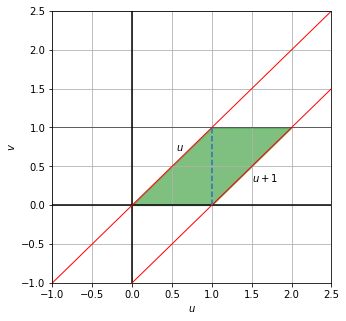
\includegraphics[scale=0.5]{../assets/support.png}
    \end{center}
    The Jacobian of the Transformation is given by,
    $|J| = \left\vert \det \begin{pmatrix}
        \frac{\partial x}{\partial u} & \frac{\partial x}{\partial v} \\
        \\
        \frac{\partial y}{\partial u} & \frac{\partial y}{\partial v}
    \end{pmatrix}\right\vert = \left | \det \begin{pmatrix}
        1 & -1 \\
        \\ 
        0 & 1 
    \end{pmatrix} \right |$ = 1
    \\
    \begin{align*}
        f_{U, V}(u, v) &= \frac{3}{2} (u - v) (v^2 + 2v) \cdot |J| \\ 
        &= \begin{cases} 
            \frac{3}{2} (u - v) (v^2 + 2v) & (u, v) \in S' \\
            0 & \text{otherwise} 
        \end{cases}
    \end{align*}
    Notice that the support $S'$ has the following region. 
    \begin{center}
        % \includegraphics*[scale=0.5]{{../assets/support.png}}
    \end{center}
    Thus, 
    \begin{align*}
        f_{U}(u) &= \int_{-\infty}^{\infty}f_{U, V}(u, v)\,dv \\ 
        &= \begin{cases}
            \int_{0}^{u} f_{U, V}(u, v)\,dv \quad & 0<u<1 \\
            \int_{u-1}^{1} f_{U, V}(u, v)\,dv  \quad & 1<u<2
        \end{cases}
    \end{align*}
    Since we're only interested in the region of $U=X+Y < 0.5$, we'll just use
    the first case.
    \begin{align*}
        f_U(u) &= \int_{0}^{u} \frac{3}{2} (u - v) (v^2 + 2v)\, dv \\
        &= \frac{3}{2} \int_{0}^{u} uv^2 + 2uv - v^3 - 2v^2\, dv \\
        &= \frac{3}{2} \int_{0}^{u} - v^3 + (u-2)v^2 + 2uv\, dv \\
        &= \frac{3}{2} \left[- \frac{1}{4}v^4 + \frac{u-2}{3}v^3 + uv^2\right]^{u}_{0}\\
        &= \frac{3}{2} \left(- \frac{1}{4}u^4 + \frac{u-2}{3}u^3 + u^3 \right)\\ 
        &= \frac{3}{2} \left(- \frac{1}{4}u^4 + \frac{1}{3}u^4 - \frac{2}{3} u^3 + u^3 \right)\\ 
        &= \frac{3}{2} \left(\frac{1}{12}u^4 + \frac{1}{3} u^3  \right)\\ 
        &= \frac{1}{8}u^4 + \frac{1}{2} u^3 \\ 
        \\
        f_U(u) &= \frac{1}{8}u^4 + \frac{1}{2} u^3  \quad 0 < u < 1 \\
    \end{align*}
    \begin{align*}
        P[X+Y < 0.5] &= \int_{0}^{0.5} f_U(u) du \\ 
        &= \int_{0}^{0.5} \frac{1}{8}u^4 + \frac{1}{2} u^3 du  \\ 
        &= \left.\frac{1}{40}u^{5} + \dfrac{1}{8}u^4 \right|_{0}^{\dfrac{1}{2}} \\ 
        &= \dfrac{1}{2^{3}\cdot 5} \cdot \dfrac{1}{2^{5}} + \dfrac{1}{2^{3}}\cdot \dfrac{1}{2^{4}} \\ 
        &= \dfrac{1}{2^{8}\cdot 5} + \dfrac{1}{2^{7}} \\ 
        &= \dfrac{1}{2^{7}} \cdot \frac{11}{10} \\ 
        &= \frac{11}{1280}
    \end{align*}

    \subsection*{2)}
    \begin{align*}
        f_{X,Y}(x, y) = \left\{ \begin{array}{cc} \frac{3}{2}x(y^2 + 2y) & 0 < x, y < 1 \\ 0 & \textrm{ otherwise} \end{array} \right.
    \end{align*}
    \begin{align*}
        f_{X}\left( x\right) &= \int _{0}^{1} f_{X,Y} (x,y) \,dy \\ 
        &= \int _{0}^{1} x\left(\frac{3}{2}y^2 + 3y\right) \,dy \\
        &= x \left[ \frac{1}{2}y^3 + \frac{3}{2} y^2 \right]^{1}_{0} \\
        &= 2x \\ \\ 
        f_X(x) &= \begin{cases}
            2x \quad & 0 < x < 1 \\ 
            0 \quad & o.w.
        \end{cases} 
    \end{align*}
    \begin{align*}
        E[X] &= \int_{0}^{1} x \cdot f_X(x) \,dx \\
        &= \int_{0}^{1} 2x^2 \,dx \\ 
        &= \left.\frac{2}{3}x^3\right|_0^1 \\
        &= \frac{2}{3}
    \end{align*}

    \subsection*{3)}
    $$Var[Y] = E[Y^2] - E[Y]^2$$

    \begin{align*}
        f_{X,Y}(x, y) = \left\{ \begin{array}{cc} \frac{3}{2}x(y^2 + 2y) & 0 < x, y < 1 \\ 0 & \textrm{ otherwise} \end{array} \right.
    \end{align*}
    Notice that the joint pdf on the support can be factorized into two parts
    $f_{X,Y}(x, y) = g(x) \cdot h(y)$, which implies that $X, Y$ are
    independent. Thus, by the definition of independence, we can get the marginal
    pdf of $Y,\ f_Y$ by deviding the joint pdf $f_{X,Y}$ with the marginal pdf
    of $X,\ f_X$, which we calculated above.
    \begin{align*}
        f_Y(y) &= \frac{f_{X, Y}(x, y)}{f_X(x)} \\ 
        &= \frac{\frac{3}{2}x(y^2 + 2y)}{2x} \\
        &= \frac{3}{4}(y^2 + 2y) \\ \\ 
        &= \begin{cases}
            \frac{3}{4}(y^2 + 2y) \quad & 0 < y < 1\\
            0 \quad & o.w.\\
        \end{cases}
    \end{align*}

    \begin{align*}
        E[Y] &= \int _{0}^{1} y \cdot f_{Y}(y)\,dy \\
            &= \int _{0}^{1}\dfrac{3}{4}y^{3}+\dfrac{3}{2}y^{2}\,dy \\
            &= \left. \dfrac{3}{16}y^{4}+\dfrac{1}{2}y^{3}\right]^1_0 \\
            &= \dfrac{3}{16}+\dfrac{1}{2} \\
            &= \dfrac{11}{16}
    \end{align*}
    
    \begin{align*}
        E\left[ Y^{2}\right] &= \int _{0}^{1}y^{2}f_{Y}\left( y\right)\,dy \\ 
        &= \int _{0}^{1}\dfrac{3}{4}y^{4}+\dfrac{3}{2}y^{3}\,dy \\
        &= \left.\dfrac{3}{20}y^{5}+\dfrac{3}{8}y^{4}\right]_{0}^{1} \\ 
        &= \dfrac{3}{20}+\dfrac{3}{8} \\ 
        &= \dfrac{6}{40}+\dfrac{15}{40} \\ 
        &= \dfrac{21}{40}
    \end{align*}

    \begin{align*}
        Var\left[Y\right] &= \dfrac{21}{40}-\left( \dfrac{11}{16}\right) ^{2} \\ 
        &= \dfrac{21}{40}-\dfrac{121}{256} \\ 
        &= \dfrac{67}{1280}
    \end{align*}

    \subsection*{4)}
    Since $X\ \ind\ Y,\ E[XY] = E[X]E[Y]$.
    \begin{align*}
        Cov(X, Y) = E[XY] - E[X] \cdot E[Y] = 0
    \end{align*}

    \subsection*{5)}
    $$Corr(X, Y) = 0 \quad (\because\ Cov(X, Y) = 0)$$

    \subsection*{6)}
    Since $0 < x < 1,\ 0 < y < 1$, and $X \ind Y$,
    \begin{align*}
        P(X > 0.5 | Y > 0.5) &= \dfrac{P\left(X > 0.5,\ Y > 0.5 \right)}{P\left(Y > 0.5 \right)} 
    \end{align*}
    \begin{align*}
        P(X > 0.5,\ Y > 0.5) &= P(X > 0.5) \cdot P(Y > 0.5) \\ 
        &= (1 - P(X \leq 0.5)) \cdot (1 - P(Y \leq 0.5)) 
    \end{align*}
    where
    \begin{align*}
        P(X \leq 0.5) &= \int_{0}^{0.5}2x \,dx \\ 
        &= \left.\frac{}{}x^2\right|^{0.5}_0 \\ 
        &= \frac{1}{4}
    \end{align*}
    \begin{align*}
        P\left( Y \leq 0.5 \right)
        &= \int _{0}^{0.5}\dfrac{3}{4}y^{2}+\dfrac{3}{2}y\,dy \\ 
        &= \left. \dfrac{1}{4}y^{3}+\dfrac{3}{4}y^{2} \right|_{0}^{\frac{1}{2}}  \\ 
        &= \dfrac{1}{32}+\dfrac{3}{16} \\ 
        &= \frac{7}{32}    
    \end{align*}
    \begin{align*}
        P(X > 0.5,\ Y > 0.5) &= \left(1-\frac{1}{4}\right)\cdot \left(1 - \frac{7}{32}\right) \\ 
        &= \frac{3}{4} \cdot \frac{25}{32} \\ 
        &= \frac{75}{128}
    \end{align*}
    \begin{align*}
        P(X > 0.5 | Y > 0.5) &= {\frac{75}{128}}\cdot{\frac{32}{25}} = \frac{3}{4} \\  
    \end{align*}

    \subsection*{7)}
    \begin{align*}
        f_{X|Y}(x|y) &= \frac{f_{X,Y}(x,y)}{f_Y(y)}, \quad 0 < x, y < 1 \\ 
        &= \frac{f_{X}(x)f_Y(y)}{f_Y(y)} \\ 
        &= f_{X}(x) \\ 
        &= 2x
    \end{align*}
    \begin{align*}
        f_{X|Y=0.25}(x) &= 2x
    \end{align*}
    \begin{align*}
        E[X|Y=0.25] &= E[X] \\ 
        &= \frac{2}{3}
    \end{align*}

\hypertarget{problem-2}{%
\section{Problem 2}\label{problem-2}}

Use Monte Carlo integration to estimate

\[\int_{-2}^{3}3x^2 + 2x\,\textrm{d}x\]

(The exact answer is 40. You don't need to rederive it.)

Use a sample size of at least \(n = 100,000\).

Let
\(u = \frac{1}{5}x + \frac{2}{5} \Leftrightarrow x = 5u - 2,\quad \frac{dx}{du} = 5\)
\begin{align*}
    \int_{-2}^{3}3x^2 + 2x\,dx &= \int_{0}^{1} (3(5u - 2)^2 + 2(5u - 2)) \frac{dx}{du} \,du  \\ 
    &= \int^{1}_{0} ( 3(25u^{2} - 20u + 4) + 10u - 4) \cdot 5\,du \\ 
    &= \int_{0}^{1}\left( 75u^{2} - 60u + 12 + 10u - 4 \right) \cdot 5\,du \\ 
    &= \int^{1}_{0} 375u^{2} - 250u + 40 \,du \\ 
    &= E[f(U)]
\end{align*}
\(\text{where } U \sim \text{Unif}(0,1)\text{ and }f(u) = 375u^{2} - 250u + 40\)

    By default, \texttt{np.random.random()} method uses Mersenne Twister
algorithm (\texttt{MT19937}) for its Pesudo Random Number
Generator(PRNG). However, the official numpy documentation recommends to
use other modern PRNG instead of \texttt{MT19937}, since
\texttt{MT19937} fails some statiscal tests and does not have any
significant advantage in its generation speed.

Therefore, for the generation of Uniform random samples, I used
Permutation Congruential Generator (\texttt{PCG64}) as recommended.

In addition, I used parallel processing to generate very large numbers
of sample. As shown in below, multi-threaded generator made a
significant improvement in speed compared to a single-threaded
generator.

Ref: https://numpy.org/doc/stable/reference/random/performance.html

    \begin{tcolorbox}[breakable, size=fbox, boxrule=1pt, pad at break*=1mm,colback=cellbackground, colframe=cellborder]
\prompt{In}{incolor}{5}{\boxspacing}
\begin{Verbatim}[commandchars=\\\{\}]
\PY{k+kn}{import} \PY{n+nn}{numpy} \PY{k}{as} \PY{n+nn}{np}
\PY{n}{rng} \PY{o}{=} \PY{n}{np}\PY{o}{.}\PY{n}{random}\PY{o}{.}\PY{n}{default\PYZus{}rng}\PY{p}{(}\PY{l+m+mi}{12}\PY{p}{)}
\PY{c+c1}{\PYZsh{} Use Permutation Congruential Generator(PCG64) instead of Mersenne Twister(MT19937)}
\end{Verbatim}
\end{tcolorbox}

    \begin{tcolorbox}[breakable, size=fbox, boxrule=1pt, pad at break*=1mm,colback=cellbackground, colframe=cellborder]
\prompt{In}{incolor}{6}{\boxspacing}
\begin{Verbatim}[commandchars=\\\{\}]
\PY{k+kn}{from} \PY{n+nn}{numpy}\PY{n+nn}{.}\PY{n+nn}{random} \PY{k+kn}{import} \PY{n}{default\PYZus{}rng}\PY{p}{,} \PY{n}{SeedSequence}
\PY{k+kn}{import} \PY{n+nn}{multiprocessing}
\PY{k+kn}{import} \PY{n+nn}{concurrent}\PY{n+nn}{.}\PY{n+nn}{futures}
\PY{k+kn}{import} \PY{n+nn}{numpy} \PY{k}{as} \PY{n+nn}{np}

\PY{k}{class} \PY{n+nc}{MultithreadedRNG}\PY{p}{:}
    \PY{k}{def} \PY{n+nf+fm}{\PYZus{}\PYZus{}init\PYZus{}\PYZus{}}\PY{p}{(}\PY{n+nb+bp}{self}\PY{p}{,} \PY{n}{n}\PY{p}{,} \PY{n}{seed}\PY{o}{=}\PY{k+kc}{None}\PY{p}{,} \PY{n}{threads}\PY{o}{=}\PY{k+kc}{None}\PY{p}{)}\PY{p}{:}
        \PY{k}{if} \PY{n}{threads} \PY{o+ow}{is} \PY{k+kc}{None}\PY{p}{:}
            \PY{n}{threads} \PY{o}{=} \PY{n}{multiprocessing}\PY{o}{.}\PY{n}{cpu\PYZus{}count}\PY{p}{(}\PY{p}{)}
        \PY{n+nb+bp}{self}\PY{o}{.}\PY{n}{threads} \PY{o}{=} \PY{n}{threads}

        \PY{n}{seq} \PY{o}{=} \PY{n}{SeedSequence}\PY{p}{(}\PY{n}{seed}\PY{p}{)}
        \PY{n+nb+bp}{self}\PY{o}{.}\PY{n}{\PYZus{}random\PYZus{}generators} \PY{o}{=} \PY{p}{[}\PY{n}{default\PYZus{}rng}\PY{p}{(}\PY{n}{s}\PY{p}{)}
                                   \PY{k}{for} \PY{n}{s} \PY{o+ow}{in} \PY{n}{seq}\PY{o}{.}\PY{n}{spawn}\PY{p}{(}\PY{n}{threads}\PY{p}{)}\PY{p}{]}

        \PY{n+nb+bp}{self}\PY{o}{.}\PY{n}{n} \PY{o}{=} \PY{n}{n}
        \PY{n+nb+bp}{self}\PY{o}{.}\PY{n}{executor} \PY{o}{=} \PY{n}{concurrent}\PY{o}{.}\PY{n}{futures}\PY{o}{.}\PY{n}{ThreadPoolExecutor}\PY{p}{(}\PY{n}{threads}\PY{p}{)}
        \PY{n+nb+bp}{self}\PY{o}{.}\PY{n}{values} \PY{o}{=} \PY{n}{np}\PY{o}{.}\PY{n}{empty}\PY{p}{(}\PY{n}{n}\PY{p}{)}
        \PY{n+nb+bp}{self}\PY{o}{.}\PY{n}{step} \PY{o}{=} \PY{n}{np}\PY{o}{.}\PY{n}{ceil}\PY{p}{(}\PY{n}{n} \PY{o}{/} \PY{n}{threads}\PY{p}{)}\PY{o}{.}\PY{n}{astype}\PY{p}{(}\PY{n}{np}\PY{o}{.}\PY{n}{int\PYZus{}}\PY{p}{)}

    \PY{k}{def} \PY{n+nf}{fill}\PY{p}{(}\PY{n+nb+bp}{self}\PY{p}{)}\PY{p}{:}
        \PY{k}{def} \PY{n+nf}{\PYZus{}fill}\PY{p}{(}\PY{n}{random\PYZus{}state}\PY{p}{,} \PY{n}{out}\PY{p}{,} \PY{n}{first}\PY{p}{,} \PY{n}{last}\PY{p}{)}\PY{p}{:}
            \PY{n}{random\PYZus{}state}\PY{o}{.}\PY{n}{random}\PY{p}{(}\PY{n}{out}\PY{o}{=}\PY{n}{out}\PY{p}{[}\PY{n}{first}\PY{p}{:}\PY{n}{last}\PY{p}{]}\PY{p}{)}

        \PY{n}{futures} \PY{o}{=} \PY{p}{\PYZob{}}\PY{p}{\PYZcb{}}
        \PY{k}{for} \PY{n}{i} \PY{o+ow}{in} \PY{n+nb}{range}\PY{p}{(}\PY{n+nb+bp}{self}\PY{o}{.}\PY{n}{threads}\PY{p}{)}\PY{p}{:}
            \PY{n}{args} \PY{o}{=} \PY{p}{(}\PY{n}{\PYZus{}fill}\PY{p}{,}
                    \PY{n+nb+bp}{self}\PY{o}{.}\PY{n}{\PYZus{}random\PYZus{}generators}\PY{p}{[}\PY{n}{i}\PY{p}{]}\PY{p}{,}
                    \PY{n+nb+bp}{self}\PY{o}{.}\PY{n}{values}\PY{p}{,}
                    \PY{n}{i} \PY{o}{*} \PY{n+nb+bp}{self}\PY{o}{.}\PY{n}{step}\PY{p}{,}
                    \PY{p}{(}\PY{n}{i} \PY{o}{+} \PY{l+m+mi}{1}\PY{p}{)} \PY{o}{*} \PY{n+nb+bp}{self}\PY{o}{.}\PY{n}{step}\PY{p}{)}
            \PY{n}{futures}\PY{p}{[}\PY{n+nb+bp}{self}\PY{o}{.}\PY{n}{executor}\PY{o}{.}\PY{n}{submit}\PY{p}{(}\PY{o}{*}\PY{n}{args}\PY{p}{)}\PY{p}{]} \PY{o}{=} \PY{n}{i}
        \PY{n}{concurrent}\PY{o}{.}\PY{n}{futures}\PY{o}{.}\PY{n}{wait}\PY{p}{(}\PY{n}{futures}\PY{p}{)}

    \PY{k}{def} \PY{n+nf+fm}{\PYZus{}\PYZus{}del\PYZus{}\PYZus{}}\PY{p}{(}\PY{n+nb+bp}{self}\PY{p}{)}\PY{p}{:}
        \PY{n+nb+bp}{self}\PY{o}{.}\PY{n}{executor}\PY{o}{.}\PY{n}{shutdown}\PY{p}{(}\PY{k+kc}{False}\PY{p}{)}
\end{Verbatim}
\end{tcolorbox}

    \begin{tcolorbox}[breakable, size=fbox, boxrule=1pt, pad at break*=1mm,colback=cellbackground, colframe=cellborder]
\prompt{In}{incolor}{7}{\boxspacing}
\begin{Verbatim}[commandchars=\\\{\}]
\PY{n}{mrng} \PY{o}{=} \PY{n}{MultithreadedRNG}\PY{p}{(}\PY{l+m+mi}{100\PYZus{}000\PYZus{}000}\PY{p}{,} \PY{n}{seed}\PY{o}{=}\PY{l+m+mi}{12}\PY{p}{)}
\end{Verbatim}
\end{tcolorbox}

    \begin{tcolorbox}[breakable, size=fbox, boxrule=1pt, pad at break*=1mm,colback=cellbackground, colframe=cellborder]
\prompt{In}{incolor}{8}{\boxspacing}
\begin{Verbatim}[commandchars=\\\{\}]
\PY{k+kn}{from} \PY{n+nn}{timeit} \PY{k+kn}{import} \PY{n}{timeit}
\PY{n+nb}{print}\PY{p}{(}\PY{l+s+s2}{\PYZdq{}}\PY{l+s+s2}{Single Thread}\PY{l+s+s2}{\PYZdq{}}\PY{p}{)}
\PY{n}{value} \PY{o}{=} \PY{n}{np}\PY{o}{.}\PY{n}{empty}\PY{p}{(}\PY{l+m+mi}{100\PYZus{}000\PYZus{}000}\PY{p}{)}
\PY{o}{\PYZpc{}}\PY{k}{timeit} rng.random(out=value)
\PY{n+nb}{print}\PY{p}{(}\PY{l+s+sa}{f}\PY{l+s+s2}{\PYZdq{}}\PY{l+s+s2}{Multi Thread (num\PYZus{}threads=}\PY{l+s+si}{\PYZob{}}\PY{n}{mrng}\PY{o}{.}\PY{n}{threads}\PY{l+s+si}{\PYZcb{}}\PY{l+s+s2}{)}\PY{l+s+s2}{\PYZdq{}}\PY{p}{)}
\PY{o}{\PYZpc{}}\PY{k}{timeit} mrng.fill()
\end{Verbatim}
\end{tcolorbox}

    \begin{Verbatim}[commandchars=\\\{\}]
Single Thread
437 ms ± 19.5 ms per loop (mean ± std. dev. of 7 runs, 1 loop each)
Multi Thread (num\_threads=8)
75.1 ms ± 1.5 ms per loop (mean ± std. dev. of 7 runs, 10 loops each)
    \end{Verbatim}

    \begin{tcolorbox}[breakable, size=fbox, boxrule=1pt, pad at break*=1mm,colback=cellbackground, colframe=cellborder]
\prompt{In}{incolor}{9}{\boxspacing}
\begin{Verbatim}[commandchars=\\\{\}]
\PY{k+kn}{from} \PY{n+nn}{tqdm} \PY{k+kn}{import} \PY{n}{tqdm}
\PY{n}{val} \PY{o}{=} \PY{l+m+mf}{0.}
\PY{n}{ests} \PY{o}{=} \PY{p}{[}\PY{p}{]}
\PY{k}{for} \PY{n}{i} \PY{o+ow}{in} \PY{n}{tqdm}\PY{p}{(}\PY{n+nb}{range}\PY{p}{(}\PY{l+m+mi}{1000}\PY{p}{)}\PY{p}{)}\PY{p}{:}
    \PY{n}{mrng}\PY{o}{.}\PY{n}{fill}\PY{p}{(}\PY{p}{)}
    \PY{n}{smpls} \PY{o}{=} \PY{n}{mrng}\PY{o}{.}\PY{n}{values}
    \PY{n}{val} \PY{o}{+}\PY{o}{=} \PY{n}{np}\PY{o}{.}\PY{n}{sum}\PY{p}{(}\PY{l+m+mi}{375} \PY{o}{*} \PY{p}{(}\PY{n}{smpls} \PY{o}{*}\PY{o}{*} \PY{l+m+mi}{2}\PY{p}{)} \PY{o}{\PYZhy{}} \PY{l+m+mi}{250} \PY{o}{*} \PY{n}{smpls} \PY{o}{+} \PY{l+m+mi}{40}\PY{p}{)}
    \PY{n}{ests}\PY{o}{.}\PY{n}{append}\PY{p}{(}\PY{n}{val} \PY{o}{/} \PY{p}{(}\PY{p}{(}\PY{n}{i}\PY{o}{+}\PY{l+m+mi}{1}\PY{p}{)} \PY{o}{*} \PY{n+nb}{int}\PY{p}{(}\PY{l+m+mf}{1e8}\PY{p}{)}\PY{p}{)}\PY{p}{)}
\end{Verbatim}
\end{tcolorbox}

    \begin{tcolorbox}[breakable, size=fbox, boxrule=1pt, pad at break*=1mm,colback=cellbackground, colframe=cellborder]
\prompt{In}{incolor}{10}{\boxspacing}
\begin{Verbatim}[commandchars=\\\{\}]
\PY{k+kn}{import} \PY{n+nn}{matplotlib}\PY{n+nn}{.}\PY{n+nn}{pyplot} \PY{k}{as} \PY{n+nn}{plt}
\PY{n}{plt}\PY{o}{.}\PY{n}{plot}\PY{p}{(}\PY{n}{ests}\PY{p}{)}
\PY{n}{plt}\PY{o}{.}\PY{n}{axhline}\PY{p}{(}\PY{l+m+mi}{40}\PY{p}{,} \PY{n}{color}\PY{o}{=}\PY{l+s+s1}{\PYZsq{}}\PY{l+s+s1}{red}\PY{l+s+s1}{\PYZsq{}}\PY{p}{,} \PY{n}{label}\PY{o}{=}\PY{l+s+s2}{\PYZdq{}}\PY{l+s+s2}{Actual value (40)}\PY{l+s+s2}{\PYZdq{}}\PY{p}{)}
\PY{n}{plt}\PY{o}{.}\PY{n}{xlabel}\PY{p}{(}\PY{l+s+s2}{\PYZdq{}}\PY{l+s+s2}{Sample size (in units of 100M=1e8)}\PY{l+s+s2}{\PYZdq{}}\PY{p}{)}
\PY{n}{plt}\PY{o}{.}\PY{n}{legend}\PY{p}{(}\PY{p}{)}
\PY{n}{plt}\PY{o}{.}\PY{n}{title}\PY{p}{(}\PY{l+s+s2}{\PYZdq{}}\PY{l+s+s2}{Monte Carlo estimate as sample size increases}\PY{l+s+s2}{\PYZdq{}}\PY{p}{)}
\PY{n}{plt}\PY{o}{.}\PY{n}{show}\PY{p}{(}\PY{p}{)}
\end{Verbatim}
\end{tcolorbox}

    \begin{center}
    \adjustimage{max size={0.6\linewidth}{0.4\paperheight}}{../assets/plot1.png}
    \end{center}
    { \hspace*{\fill} \\}
    
    \begin{tcolorbox}[breakable, size=fbox, boxrule=1pt, pad at break*=1mm,colback=cellbackground, colframe=cellborder]
\prompt{In}{incolor}{11}{\boxspacing}
\begin{Verbatim}[commandchars=\\\{\}]
\PY{n+nb}{print}\PY{p}{(}\PY{l+s+sa}{f}\PY{l+s+s2}{\PYZdq{}}\PY{l+s+si}{\PYZob{}}\PY{l+s+s1}{\PYZsq{}}\PY{l+s+s1}{Monte Carlo estimate }\PY{l+s+s1}{\PYZsq{}}\PY{l+s+si}{:}\PY{l+s+s2}{ \PYZlt{}21}\PY{l+s+si}{\PYZcb{}}\PY{l+s+s2}{ = }\PY{l+s+si}{\PYZob{}}\PY{n}{ests}\PY{p}{[}\PY{o}{\PYZhy{}}\PY{l+m+mi}{1}\PY{p}{]}\PY{l+s+si}{\PYZcb{}}\PY{l+s+s2}{\PYZdq{}}\PY{p}{)}
\PY{n+nb}{print}\PY{p}{(}\PY{l+s+sa}{f}\PY{l+s+s2}{\PYZdq{}}\PY{l+s+si}{\PYZob{}}\PY{l+s+s1}{\PYZsq{}}\PY{l+s+s1}{Theoretical value }\PY{l+s+s1}{\PYZsq{}}\PY{l+s+si}{:}\PY{l+s+s2}{ \PYZlt{}21}\PY{l+s+si}{\PYZcb{}}\PY{l+s+s2}{ = }\PY{l+s+si}{\PYZob{}}\PY{l+m+mi}{40}\PY{l+s+si}{\PYZcb{}}\PY{l+s+s2}{\PYZdq{}}\PY{p}{)}
\end{Verbatim}
\end{tcolorbox}

    \begin{Verbatim}[commandchars=\\\{\}]
Monte Carlo estimate  = 40.0000533971071
Theoretical value     = 40
    \end{Verbatim}

    \hypertarget{problem-3}{%
\section{Problem 3}\label{problem-3}}

Use Monte Carlo integration to estimate

\[\int_{0}^{\infty}\int_{0}^{1}\frac{xy}{1 + x^4}\,\textrm{d}y\textrm{d}x\]

(The exact answer is \(\pi/8\). You don't need to rederive it.)

Use a sample size of at least \(n = 100,000\).

    Let $z = \frac{x}{1+x} = \frac{1}{\frac{1}{x} + 1} \Leftrightarrow x =
\dfrac{z}{1-z}, \quad \dfrac{dx}{dz} = \dfrac{1}{\left( 1-z\right) ^{2}}$

    Notice that \(0 < x < \infty \Leftrightarrow 0 < z < 1\) since
\[\lim_{x \rightarrow 0+} \frac{1}{\frac{1}{x} + 1} = 0, \quad 
    \lim_{x \rightarrow \infty} \frac{1}{\frac{1}{x} + 1} = 1\]
\begin{align*}
    \int_{0}^{\infty}\int_{0}^{1}\frac{xy}{1 + x^4}\,\textrm{d}y\textrm{d}x &= 
    \int_{0}^{1} \int_{0}^{1} \dfrac{\dfrac{z}{1-z}y}{1+\left( \dfrac{z}{1-z}\right) ^{4}}\cdot \dfrac{1}{\left( 1-z\right) ^{2}}\,dx\,dz \\
    &= \int_{0}^{1} \int_{0}^{1} \dfrac{\dfrac{z}{(1-z)^3}}{1+\dfrac{z^{4}}{\left( 1-z\right) ^{4}}}y \,dz\,dy \\
    &= \int_{0}^{1} \int^{1}_{0} \dfrac{\left( 1-z\right) \cdot z}{\left( 1-z\right) ^{4}+z^{4}}y \,dz\,dy \\ 
    &= E[f(Z) \cdot Y]  
\end{align*} where
\(Y,\ Z \overset{\mathrm{\text{iid}}}{\sim} \text{Unif}(0, 1)\) and
\(f(z) = \dfrac{\left(1-z\right) \cdot z}{\left( 1-z\right)^{4}+z^{4}}\)

    \begin{tcolorbox}[breakable, size=fbox, boxrule=1pt, pad at break*=1mm,colback=cellbackground, colframe=cellborder]
\prompt{In}{incolor}{12}{\boxspacing}
\begin{Verbatim}[commandchars=\\\{\}]
\PY{n}{u1} \PY{o}{=} \PY{n}{mrng}\PY{o}{.}\PY{n}{values}\PY{o}{.}\PY{n}{copy}\PY{p}{(}\PY{p}{)}
\PY{n}{mrng}\PY{o}{.}\PY{n}{fill}\PY{p}{(}\PY{p}{)}
\PY{n}{u2} \PY{o}{=} \PY{n}{mrng}\PY{o}{.}\PY{n}{values}\PY{o}{.}\PY{n}{copy}\PY{p}{(}\PY{p}{)}
\PY{n}{est} \PY{o}{=} \PY{n}{np}\PY{o}{.}\PY{n}{mean}\PY{p}{(}\PY{p}{(}\PY{p}{(}\PY{p}{(}\PY{l+m+mi}{1}\PY{o}{\PYZhy{}}\PY{n}{u1}\PY{p}{)} \PY{o}{*} \PY{n}{u1}\PY{p}{)} \PY{o}{/} \PY{p}{(}\PY{p}{(}\PY{l+m+mi}{1}\PY{o}{\PYZhy{}}\PY{n}{u1}\PY{p}{)} \PY{o}{*}\PY{o}{*} \PY{l+m+mi}{4} \PY{o}{+} \PY{n}{u1} \PY{o}{*}\PY{o}{*} \PY{l+m+mi}{4}\PY{p}{)}\PY{p}{)} \PY{o}{*} \PY{n}{u2}\PY{p}{)}
\PY{n+nb}{print}\PY{p}{(}\PY{l+s+sa}{f}\PY{l+s+s2}{\PYZdq{}}\PY{l+s+si}{\PYZob{}}\PY{l+s+s1}{\PYZsq{}}\PY{l+s+s1}{Monte Carlo estimate }\PY{l+s+s1}{\PYZsq{}} \PY{l+s+si}{:}\PY{l+s+s2}{ \PYZlt{}21}\PY{l+s+si}{\PYZcb{}}\PY{l+s+s2}{ = }\PY{l+s+si}{\PYZob{}}\PY{n}{est}\PY{l+s+si}{\PYZcb{}}\PY{l+s+s2}{\PYZdq{}}\PY{p}{)}
\PY{n+nb}{print}\PY{p}{(}\PY{l+s+sa}{f}\PY{l+s+s2}{\PYZdq{}}\PY{l+s+si}{\PYZob{}}\PY{l+s+s1}{\PYZsq{}}\PY{l+s+s1}{Theoretical value }\PY{l+s+s1}{\PYZsq{}} \PY{l+s+si}{:}\PY{l+s+s2}{ \PYZlt{}21}\PY{l+s+si}{\PYZcb{}}\PY{l+s+s2}{ = }\PY{l+s+si}{\PYZob{}}\PY{n}{np}\PY{o}{.}\PY{n}{pi} \PY{o}{/} \PY{l+m+mi}{8}\PY{l+s+si}{\PYZcb{}}\PY{l+s+s2}{\PYZdq{}}\PY{p}{)}
\end{Verbatim}
\end{tcolorbox}

    \begin{Verbatim}[commandchars=\\\{\}]
Monte Carlo estimate  = 0.39275503717035704
Theoretical value     = 0.39269908169872414
    \end{Verbatim}

    \hypertarget{problem-4}{%
\section{Problem 4}\label{problem-4}}

Let \(U \sim U(0, 1)\) and \(X = 1 - U\). Use Monte Carlo simulation to
confirm that

\[\mathbb{E}[X] = \frac{1}{2} \:\textrm{ and }\: \textrm{Var}[X] = \frac{1}{12} \:\textrm{ and }\: \textrm{Cov}[U, X] = -\frac{1}{12}\]

Use a sample size of at least \(n = 100,000\).

    \begin{tcolorbox}[breakable, size=fbox, boxrule=1pt, pad at break*=1mm,colback=cellbackground, colframe=cellborder]
\prompt{In}{incolor}{13}{\boxspacing}
\begin{Verbatim}[commandchars=\\\{\}]
\PY{n}{u} \PY{o}{=} \PY{n}{mrng}\PY{o}{.}\PY{n}{values}
\PY{n}{x} \PY{o}{=} \PY{l+m+mi}{1} \PY{o}{\PYZhy{}} \PY{n}{u}
\end{Verbatim}
\end{tcolorbox}

    \begin{tcolorbox}[breakable, size=fbox, boxrule=1pt, pad at break*=1mm,colback=cellbackground, colframe=cellborder]
\prompt{In}{incolor}{14}{\boxspacing}
\begin{Verbatim}[commandchars=\\\{\}]
\PY{n+nb}{print}\PY{p}{(}\PY{l+s+s2}{\PYZdq{}}\PY{l+s+s2}{Monte Carlo estimates}\PY{l+s+s2}{\PYZdq{}}\PY{p}{)}
\PY{n+nb}{print}\PY{p}{(}\PY{l+s+s2}{\PYZdq{}}\PY{l+s+s2}{\PYZhy{}\PYZhy{}\PYZhy{}}\PY{l+s+s2}{\PYZdq{}} \PY{o}{*} \PY{l+m+mi}{15}\PY{p}{)}
\PY{n+nb}{print}\PY{p}{(}\PY{l+s+sa}{f}\PY{l+s+s2}{\PYZdq{}}\PY{l+s+si}{\PYZob{}}\PY{l+s+s1}{\PYZsq{}}\PY{l+s+s1}{E[X] }\PY{l+s+s1}{\PYZsq{}} \PY{l+s+si}{:}\PY{l+s+s2}{ \PYZlt{}10}\PY{l+s+si}{\PYZcb{}}\PY{l+s+s2}{ = }\PY{l+s+si}{\PYZob{}}\PY{n}{np}\PY{o}{.}\PY{n}{mean}\PY{p}{(}\PY{n}{x}\PY{p}{)}\PY{l+s+si}{\PYZcb{}}\PY{l+s+s2}{\PYZdq{}}\PY{p}{)}
\PY{n+nb}{print}\PY{p}{(}\PY{l+s+sa}{f}\PY{l+s+s2}{\PYZdq{}}\PY{l+s+si}{\PYZob{}}\PY{l+s+s1}{\PYZsq{}}\PY{l+s+s1}{Var[X] }\PY{l+s+s1}{\PYZsq{}}\PY{l+s+si}{:}\PY{l+s+s2}{ \PYZlt{}10}\PY{l+s+si}{\PYZcb{}}\PY{l+s+s2}{ = }\PY{l+s+si}{\PYZob{}}\PY{n}{np}\PY{o}{.}\PY{n}{cov}\PY{p}{(}\PY{n}{u}\PY{p}{,}\PY{n}{x}\PY{p}{)}\PY{p}{[}\PY{l+m+mi}{0}\PY{p}{,}\PY{l+m+mi}{0}\PY{p}{]}\PY{l+s+si}{\PYZcb{}}\PY{l+s+s2}{\PYZdq{}}\PY{p}{)}
\PY{n+nb}{print}\PY{p}{(}\PY{l+s+sa}{f}\PY{l+s+s2}{\PYZdq{}}\PY{l+s+si}{\PYZob{}}\PY{l+s+s1}{\PYZsq{}}\PY{l+s+s1}{Cov[U, X] }\PY{l+s+s1}{\PYZsq{}}\PY{l+s+si}{:}\PY{l+s+s2}{ \PYZlt{}10}\PY{l+s+si}{\PYZcb{}}\PY{l+s+s2}{ = }\PY{l+s+si}{\PYZob{}}\PY{n}{np}\PY{o}{.}\PY{n}{cov}\PY{p}{(}\PY{n}{u}\PY{p}{,}\PY{n}{x}\PY{p}{)}\PY{p}{[}\PY{l+m+mi}{0}\PY{p}{,}\PY{l+m+mi}{1}\PY{p}{]}\PY{l+s+si}{\PYZcb{}}\PY{l+s+s2}{\PYZdq{}}\PY{p}{)}
\PY{n+nb}{print}\PY{p}{(}\PY{l+s+s2}{\PYZdq{}}\PY{l+s+s2}{\PYZhy{}\PYZhy{}\PYZhy{}}\PY{l+s+s2}{\PYZdq{}} \PY{o}{*} \PY{l+m+mi}{15}\PY{p}{,} \PY{l+s+s2}{\PYZdq{}}\PY{l+s+se}{\PYZbs{}n}\PY{l+s+s2}{\PYZdq{}}\PY{p}{)}
\PY{n+nb}{print}\PY{p}{(}\PY{l+s+s2}{\PYZdq{}}\PY{l+s+s2}{Theoretical values}\PY{l+s+s2}{\PYZdq{}}\PY{p}{)}
\PY{n+nb}{print}\PY{p}{(}\PY{l+s+s2}{\PYZdq{}}\PY{l+s+s2}{\PYZhy{}\PYZhy{}\PYZhy{}}\PY{l+s+s2}{\PYZdq{}} \PY{o}{*} \PY{l+m+mi}{15}\PY{p}{)}
\PY{n+nb}{print}\PY{p}{(}\PY{l+s+sa}{f}\PY{l+s+s2}{\PYZdq{}}\PY{l+s+si}{\PYZob{}}\PY{l+s+s1}{\PYZsq{}}\PY{l+s+s1}{E[X] }\PY{l+s+s1}{\PYZsq{}} \PY{l+s+si}{:}\PY{l+s+s2}{ \PYZlt{}10}\PY{l+s+si}{\PYZcb{}}\PY{l+s+s2}{ = }\PY{l+s+si}{\PYZob{}}\PY{l+m+mi}{1}\PY{o}{/}\PY{l+m+mi}{2}\PY{l+s+si}{\PYZcb{}}\PY{l+s+s2}{\PYZdq{}}\PY{p}{)}
\PY{n+nb}{print}\PY{p}{(}\PY{l+s+sa}{f}\PY{l+s+s2}{\PYZdq{}}\PY{l+s+si}{\PYZob{}}\PY{l+s+s1}{\PYZsq{}}\PY{l+s+s1}{Var[X] }\PY{l+s+s1}{\PYZsq{}}\PY{l+s+si}{:}\PY{l+s+s2}{ \PYZlt{}10}\PY{l+s+si}{\PYZcb{}}\PY{l+s+s2}{ = }\PY{l+s+si}{\PYZob{}}\PY{l+m+mi}{1}\PY{o}{/}\PY{l+m+mi}{12}\PY{l+s+si}{\PYZcb{}}\PY{l+s+s2}{\PYZdq{}}\PY{p}{)}
\PY{n+nb}{print}\PY{p}{(}\PY{l+s+sa}{f}\PY{l+s+s2}{\PYZdq{}}\PY{l+s+si}{\PYZob{}}\PY{l+s+s1}{\PYZsq{}}\PY{l+s+s1}{Cov[U, X] }\PY{l+s+s1}{\PYZsq{}}\PY{l+s+si}{:}\PY{l+s+s2}{ \PYZlt{}10}\PY{l+s+si}{\PYZcb{}}\PY{l+s+s2}{ = }\PY{l+s+si}{\PYZob{}}\PY{o}{\PYZhy{}}\PY{l+m+mi}{1}\PY{o}{/}\PY{l+m+mi}{12}\PY{l+s+si}{\PYZcb{}}\PY{l+s+s2}{\PYZdq{}}\PY{p}{)}
\end{Verbatim}
\end{tcolorbox}

    \begin{Verbatim}[commandchars=\\\{\}]
Monte Carlo estimates
---------------------------------------------
E[X]       = 0.4999481238364926
Var[X]     = 0.08332875314388954
Cov[U, X]  = -0.08332875314388954
---------------------------------------------

Theoretical values
---------------------------------------------
E[X]       = 0.5
Var[X]     = 0.08333333333333333
Cov[U, X]  = -0.08333333333333333
    \end{Verbatim}

    \hypertarget{problem-5}{%
\section{Problem 5}\label{problem-5}}

Let \(U_1\) and \(U_2\) be i.i.d. uniform random variables on
\((0, 1)\). Define \(X = \textrm{max}(U_1, U_2)\). Derive the following
by hand and then use Monte carlo simulation to estimate them:

\begin{enumerate}
\def\labelenumi{\arabic{enumi})}
\item
  \(\mathbb{E}[X]\)
\item
  \(\mathbb{P}[X < 0.25]\)
\end{enumerate}

Use a sample size of at least \(n = 100,000\) for each part.

    \[X = \max(U_{1},U_{2}), \quad \text{where } U_{1},U_{2} \overset{\text{iid}}{\sim} \text{Unif}\left( 0,1\right)\]

    \begin{align*}
    P(X \leq x) &= P(\max \left( U_{1},U_{2}\right) \leq x)  \\ 
    &= P(U_{1} \leq x) \cdot P\left( U_{2}\leq x\right)  \\ 
    &= \int _{0}^{x}1\,du_1 \cdot \int _{0}^{x}1\,du_{2} \\ 
    &= x^2 
\end{align*} By definition of cdf, \[F_X(x) = P(X \leq x) = 
\begin{cases}
    1 & 1 \leq x \\
    x^2 & 0 < x < 1 \\ 
    0 & x \leq 0 \\
\end{cases}\]\\
and the pdf is \[f_X(x) = F'_X(x) = 
\begin{cases}
    2x & 0 < x < 1 \\
    0 & o.w. \\
\end{cases}\]

    \hypertarget{section}{%
\subsubsection*{1)}\label{section}}

\begin{align*}
    E[X] &= \int_{0}^{1}x f_X(x) \,dx \\
    &= \int_{0}^{1} 2x^2 \,dx \\
    &= \left. \frac{2}{3}x^3 \right|^1_0  \\ 
    &= \frac{2}{3} \\
\end{align*}

    \hypertarget{section}{%
\subsubsection*{2)}\label{section}}

\[P(X \leq 0.25) = F_X\left(\frac{1}{4}\right) = \frac{1}{16}\]

    \begin{tcolorbox}[breakable, size=fbox, boxrule=1pt, pad at break*=1mm,colback=cellbackground, colframe=cellborder]
\prompt{In}{incolor}{15}{\boxspacing}
\begin{Verbatim}[commandchars=\\\{\}]
\PY{n}{x} \PY{o}{=} \PY{n}{np}\PY{o}{.}\PY{n}{max}\PY{p}{(}\PY{p}{[}\PY{n}{u1}\PY{p}{,} \PY{n}{u2}\PY{p}{]}\PY{p}{,} \PY{n}{axis}\PY{o}{=}\PY{l+m+mi}{0}\PY{p}{)}
\end{Verbatim}
\end{tcolorbox}

    \begin{tcolorbox}[breakable, size=fbox, boxrule=1pt, pad at break*=1mm,colback=cellbackground, colframe=cellborder]
\prompt{In}{incolor}{16}{\boxspacing}
\begin{Verbatim}[commandchars=\\\{\}]
\PY{n+nb}{print}\PY{p}{(}\PY{l+s+sa}{f}\PY{l+s+s2}{\PYZdq{}}\PY{l+s+si}{\PYZob{}}\PY{l+s+s1}{\PYZsq{}}\PY{l+s+s1}{Monte Carlo estimate }\PY{l+s+s1}{\PYZsq{}}\PY{l+s+si}{:}\PY{l+s+s2}{ \PYZlt{}21}\PY{l+s+si}{\PYZcb{}}\PY{l+s+s2}{\PYZdq{}} \PY{o}{+} \PY{l+s+sa}{f}\PY{l+s+s2}{\PYZdq{}}\PY{l+s+s2}{= }\PY{l+s+si}{\PYZob{}}\PY{n}{np}\PY{o}{.}\PY{n}{mean}\PY{p}{(}\PY{n}{x}\PY{p}{)}\PY{l+s+si}{\PYZcb{}}\PY{l+s+s2}{\PYZdq{}}\PY{p}{)}
\PY{n+nb}{print}\PY{p}{(}\PY{l+s+sa}{f}\PY{l+s+s2}{\PYZdq{}}\PY{l+s+si}{\PYZob{}}\PY{l+s+s1}{\PYZsq{}}\PY{l+s+s1}{Theoretical value }\PY{l+s+s1}{\PYZsq{}}\PY{l+s+si}{:}\PY{l+s+s2}{ \PYZlt{}21}\PY{l+s+si}{\PYZcb{}}\PY{l+s+s2}{\PYZdq{}} \PY{o}{+} \PY{l+s+sa}{f}\PY{l+s+s2}{\PYZdq{}}\PY{l+s+s2}{= }\PY{l+s+si}{\PYZob{}}\PY{l+m+mi}{2}\PY{o}{/}\PY{l+m+mi}{3}\PY{l+s+si}{\PYZcb{}}\PY{l+s+s2}{\PYZdq{}}\PY{p}{)}
\end{Verbatim}
\end{tcolorbox}

    \begin{Verbatim}[commandchars=\\\{\}]
Monte Carlo estimate = 0.66668394507005
Theoretical value    = 0.6666666666666666
    \end{Verbatim}

    \begin{tcolorbox}[breakable, size=fbox, boxrule=1pt, pad at break*=1mm,colback=cellbackground, colframe=cellborder]
\prompt{In}{incolor}{17}{\boxspacing}
\begin{Verbatim}[commandchars=\\\{\}]
\PY{n+nb}{print}\PY{p}{(}\PY{l+s+sa}{f}\PY{l+s+s2}{\PYZdq{}}\PY{l+s+si}{\PYZob{}}\PY{l+s+s1}{\PYZsq{}}\PY{l+s+s1}{Monte Carlo estimate }\PY{l+s+s1}{\PYZsq{}}\PY{l+s+si}{:}\PY{l+s+s2}{ \PYZlt{}21}\PY{l+s+si}{\PYZcb{}}\PY{l+s+s2}{\PYZdq{}} \PY{o}{+} \PY{l+s+sa}{f}\PY{l+s+s2}{\PYZdq{}}\PY{l+s+s2}{= }\PY{l+s+si}{\PYZob{}}\PY{n}{np}\PY{o}{.}\PY{n}{mean}\PY{p}{(}\PY{n}{x} \PY{o}{\PYZlt{}} \PY{l+m+mf}{0.25}\PY{p}{)}\PY{l+s+si}{\PYZcb{}}\PY{l+s+s2}{\PYZdq{}}\PY{p}{)}
\PY{n+nb}{print}\PY{p}{(}\PY{l+s+sa}{f}\PY{l+s+s2}{\PYZdq{}}\PY{l+s+si}{\PYZob{}}\PY{l+s+s1}{\PYZsq{}}\PY{l+s+s1}{Theoretical value }\PY{l+s+s1}{\PYZsq{}}\PY{l+s+si}{:}\PY{l+s+s2}{ \PYZlt{}21}\PY{l+s+si}{\PYZcb{}}\PY{l+s+s2}{\PYZdq{}} \PY{o}{+} \PY{l+s+sa}{f}\PY{l+s+s2}{\PYZdq{}}\PY{l+s+s2}{= }\PY{l+s+si}{\PYZob{}}\PY{l+m+mi}{1}\PY{o}{/}\PY{l+m+mi}{16}\PY{l+s+si}{\PYZcb{}}\PY{l+s+s2}{\PYZdq{}}\PY{p}{)}
\end{Verbatim}
\end{tcolorbox}

    \begin{Verbatim}[commandchars=\\\{\}]
Monte Carlo estimate = 0.06248674
Theoretical value    = 0.0625
    \end{Verbatim}

    % Add a bibliography block to the postdoc
    
\end{document}
